\documentclass[10pt,letterpaper]{article}
\usepackage[margin=0.62in]{geometry}
\usepackage[T1]{fontenc}
\usepackage{lmodern,booktabs,microtype,xcolor,graphicx}
\usepackage[hidelinks]{hyperref}
\pagestyle{empty}
\setlength{\parindent}{0pt}
\setlength{\parskip}{4pt}
\begin{document}
{\LARGE\bfseries Exp 2: Ten Writers}\hfill{\small 26 September 2026 (UTC)}\\[3pt]
{\large Hidden editorial style: context versus weights}\\[4pt]
\textbf{The endpoint comparison between the live arms is inconclusive.} After 480 review opportunities, the paired weights-minus-context
gap is \textbf{-1.2 [-4.0, +1.5] percentage points} (95\% prompt bootstrap interval).
Valid submissions follow 95.8\% of rules for weights versus 89.1\% for context,
but submission validity is 88.5\% versus 96.6\%. A pointwise advantage is already present at 15 edits. No lasting crossover is established. The comparison at 30 edits is inconclusive.
This compares complete learning workflows with separate evolving data pools.

\textbf{Experiment.} Ten concurrent Qwen3-8B tool-using writers per arm draft, check,
revise and submit 120--350 word stories. The fixed Inkling editor applies eight
private rules. Four rounds produce 1440 live sessions and 1365 valid edited
targets across three arms: no feedback, retrieved examples in an 8k-token context,
and rank-16 LoRA retrained from base. Learning targets are replay-validated edited
tool trajectories. Writer and editor versions are separate attributed Sun commits.

\begin{minipage}[c]{0.64\linewidth}
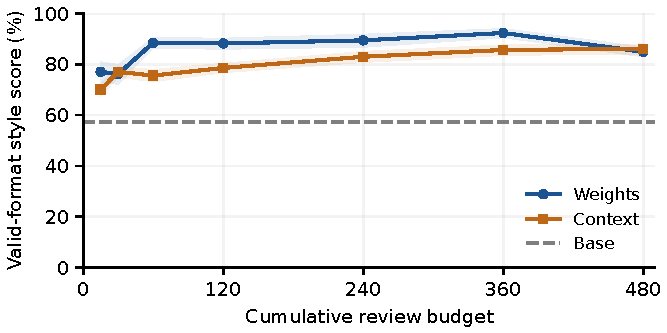
\includegraphics[width=\linewidth]{learning_curve.pdf}
\end{minipage}\hfill
\begin{minipage}[c]{0.33\linewidth}
\centering\small
\begin{tabular}{rrrr}\toprule
Reviews & Rows & Ctx. & Wts.\\\midrule
15 & 15 & 70.0 & 77.0 \\
30 & 30 & 77.0 & 76.1 \\
60 & 60 & 75.5 & 88.5 \\
120 & 116 & 78.5 & 88.2 \\
240 & 226 & 82.9 & 89.4 \\
360 & 338 & 85.6 & 92.3 \\
480 & 451 & 86.1 & 84.9 \\
\bottomrule\end{tabular}\\[4pt]
\footnotesize Scores are percentages; base is 57.1\%. Bands show 95\% intervals.
Rows are usable LoRA targets. Budgets 15--60
count valid edits. Endpoint weights average three training seeds; earlier points use one.
Endpoint seed means span 83.1--87.5\%.
\end{minipage}

\textbf{Which editor?} Using 460 matched base drafts and three seeds per editor,
opposite-editor adapters yield an A-style advantage of +80.3 [+78.3, +82.3] pp for LoRA-A over LoRA-B, and a
B-style advantage of +83.1 [+80.8, +85.4] pp for LoRA-B over LoRA-A, scored on the three flipped
rules. Edited versus unedited-target SFT differs by +33.5 [+31.8, +35.2] pp on guide A.
On the shared A-edited archive, weights score 91.8\% versus 78.2\% for context,
an endpoint gap of +13.7 [+11.4, +16.0] pp.

\textbf{Can edits rank drafts?} Best-of-4 selection by words kept changes hidden-rule
compliance for A by +3.6 [+2.8, +4.4] pp versus a uniform choice on the same candidate pools
(96 held-out prompts; valid unique drafts, subset-averaged, uniform ties). An oracle selecting by
the secret score gains +10.3 [+9.8, +10.9] pp. Selection uses the original drafts' scores.
Mean story length changes by +1.8 words.
Kept ignores pure insertions; insertion-aware edit distance is retained in the data.

\textbf{Measurement and limits.} Evaluation uses 96 held-out prompts, four samples
each, with 48 prompts from unseen genres. Score is format validity times the share
of applicable rules passed, computed by fixed regex/token checks and a pinned
spaCy tagger. Intervals resample paired prompt means 10,000 times and are conditional
on the collected training data; intervals across budgets are pointwise, without
multiple-comparison correction. Calibration edited scores average 97.3\% (A) and 99.4\% (B).
There is no completed human smoke test or blind prose-quality evaluation;
this tests recovery of planted rules, not literary taste. Raw-example context, one
live trajectory per arm, heuristic checks, and imperfect edits limit generalization.
Best-of-4 is a selection test, not reward-based training.

\vfill
{\footnotesize\color{gray}Run: \texttt{ten-writers-20260926-inkling}. Estimated token charges: \$89.80
(not a settled invoice). Reproduce with \texttt{analyze.py}; raw samples, training
manifests, costs and Sun provenance are retained under \texttt{runs/}.
Main-run wall time: 3.1 hours.}
\end{document}
